\section{Results}

\subsection{Accession-aligned abundance improves on descriptive comparators}

The full-abundance LOGO classifier has equal-cohort macro AUROC 0.9343
and separately computed pooled AUROC 0.9555. These are different
estimands: a cohort-average transfer result and a cross-model pooled
ranking statistic. Macro and pooled ECE are 0.1193 and 0.1100,
respectively. The within-cohort AUROCs range from 0.8485 (CCRCC) and
0.8610 (PDAC) through 0.9184 (UCEC) and 0.9809 (HNSCC) to 0.9974
(LSCC) and 0.9998 (LUAD) (Figure~\ref{fig:transfer}).

The missingness comparator has macro/pooled AUROC 0.5445/0.5116, while
the three reference-normalized global summaries reach 0.8172/0.8492.
Thus abundance performs better than either comparator at both levels
of aggregation, but missingness is not exactly uninformative in every
cohort. The high-dimensional model's increment over the three-summary
model is 0.1172 macro or 0.1063 pooled (Figure~\ref{fig:ladder}).
Neither increment is an identified contribution of protein-specific
biology. AUROC differences do not decompose the sources of a signal,
and these summaries are not raw signal-depth measurements.
The first-accession-consistent-gene sensitivity has macro/pooled LOGO
AUROC 0.9329/0.9557, close to the primary accession-aligned analysis
(SI Table~S4).
This is a mapping robustness check on the same samples, not replication.
The identity audit in SI Section S1 is part of the result boundary: the six
HNSCC ``.C'' samples are source-defined cored normals, the corrected manifest
contains 1,191 samples from 719 cohort-scoped patients, and the primary matrix
contains 8,906 stable ENSP accessions. The retired 9,675-name first-protein
mapping selected different stable accessions for 1,234 names; the 8,441-name
analysis is therefore a consistent-accession sensitivity, not an independent
cohort.
Table~\ref{tab:paircounts} gives the corrected tissue composition, and
Figure~\ref{fig:design} links those samples to the three evaluation units.
Neither source-defined normal tissue nor a schematic grouping rule is an
independent clinical validation cohort.

\begin{figure}[tbp]
\centering
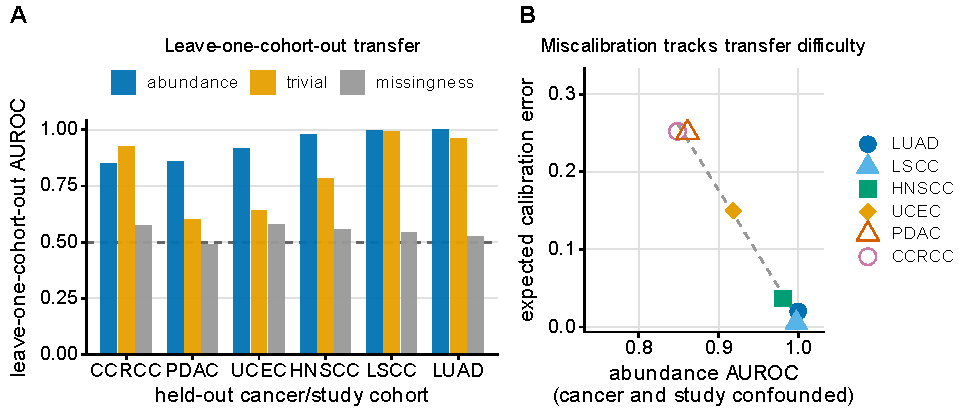
\includegraphics[width=\linewidth]{figures/b28_F1_transfer.pdf}
\caption{Heterogeneous transfer on the corrected six-cohort matrix.
(A) Within-cohort LOGO AUROC for accession-aligned abundance (blue),
three global summaries (orange) and missingness (grey). The dashed line
marks chance ranking. (B) Each cohort's abundance AUROC and ten-bin ECE.
Low-AUROC cohorts have larger calibration errors in this particular
analysis, but no deterministic relation or causal mechanism is inferred.
Each point is a cancer/study cohort; cancer type and study are confounded,
and a cohort is not asserted to be a single acquisition run.}
\label{fig:transfer}
\end{figure}

\begin{figure}[tbp]
\centering
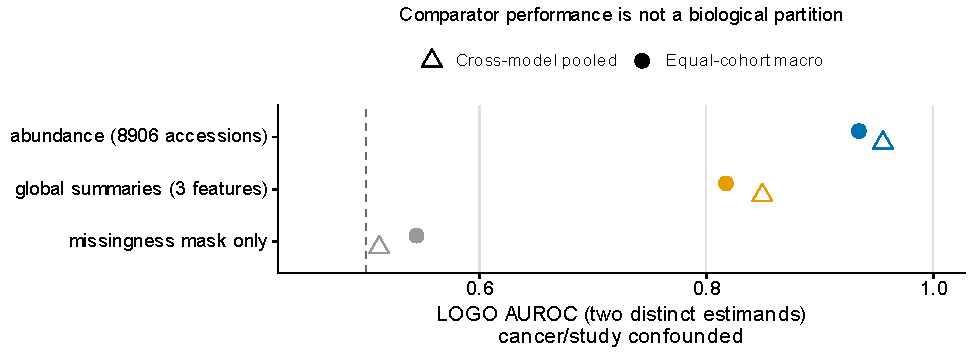
\includegraphics[width=\linewidth]{figures/b28_F2_signal_ladder.pdf}
\caption{Comparator performance is not a biological signal partition.
Filled circles show equal-cohort macro AUROC; open triangles show the
separately computed pooled AUROC, which includes cross-cohort pairs of
scores from different fitted models. Missingness, three global summaries
and 8,906-accession abundance yield macro/pooled values
0.5445/0.5116, 0.8172/0.8492 and 0.9343/0.9555, respectively.
No historical bootstrap whiskers or biological percentages are reused.
Cancer type and study remain confounded.}
\label{fig:ladder}
\end{figure}

\subsection{Calibration error concentrates on harder held-out cohorts}

The three highest-AUROC cohorts have ECE 0.0057 (LSCC), 0.0203 (LUAD)
and 0.0368 (HNSCC). ECE is higher in UCEC (0.1501), PDAC (0.2506)
and CCRCC (0.2522). The reliability curves and probability-error
metrics indicate heterogeneous calibration, not uniform unreliability.
An AUROC--ECE association in six selected cohorts does not show that
poor discrimination forces confident errors. Nor does it distinguish
tissue biology from acquisition differences. Brier scores and log-loss
for the same prediction rows are reported in SI Tables~S1--S3, with their
definitions in SI Section S2. For abundance, CCRCC and PDAC have Brier
scores 0.2245 and 0.2533 and log-loss 0.8162 and 0.7602, compared with
0.0064 and 0.0048, and 0.0253 and 0.0338, for LUAD and LSCC
(SI Table~S1). These complementary errors support the cohort-resolved
description; their relation to ECE is not a mathematical necessity.
All three tables use the same stored predictions, not additional prediction
runs.

\subsection{Random and patient-grouped CV differ from cohort transfer}

Sample CV has macro/pooled AUROC 0.9909/0.9942, and true-patient-grouped
CV has 0.9916/0.9944 (Table~\ref{tab:protocol}). Compared with LOGO, the
sample-CV advantage is 0.0565 macro and 0.0386 pooled. Patient-CV
advantages are 0.0572 macro and 0.0389 pooled. Sample minus patient CV
is $-0.0007$ macro and $-0.0003$ pooled. Preventing patient crossings
therefore does not erase the observed protocol gap in this matrix.
This finding does not isolate a batch effect or establish that patient
structure can never affect performance under another design.

Within fixed cohorts, paired resampling of patients' stored predictions
gives a 0.0442--0.0703 percentile range for the macro sample-minus-LOGO
contrast and 0.0305--0.0478 for its pooled counterpart. These conditional
mixture-sensitivity ranges omit model-refit variability and future-study
uncertainty. They cannot be substituted for a general cross-study CI.
The paired patient draws and their shared protocol contrasts are documented
in SI Table~S7 and Section S5; the ranges are conditional on the corrected patient keys,
not on the historical 723-key partition.

Pooled ECE is 0.0199 for sample CV and 0.0135 for patient CV, compared
with 0.1100 for LOGO. The corresponding macro ECE values are
0.0269, 0.0219 and 0.1193. Figure~\ref{fig:calibration} displays the
reliability curves and pooled calibration errors. The fold scatter in
Figure~\ref{fig:protocol} shows that the difference also concerns
heterogeneity: cohort holdout produces a wider spread of transfer
performance. Those folds have overlapping training sets and are not
independent statistical replicates.

\begin{table}[tbp]
\centering
\caption{Corrected patient and tissue composition. Nonmalignant samples
include both adjacent-normal and HNSCC cored-normal samples. ``Both''
counts patients with at least one sample of each class, not one-to-one
sample pairs. The six HNSCC cored samples are included in its 72 normals.}
\label{tab:paircounts}
\begin{tabular}{lrrrr}
\hline
Cohort & Samples & Tumor/normal & Patients & Both \\
\hline
\tableinput{tables/cohort_rows.tex}
\hline
\end{tabular}
\end{table}

\begin{table}[tbp]
\centering
\caption{Three protocols on the same corrected accession matrix.
Macro is the equal-weight mean of six within-cohort metrics, not the
mean of five CV-fold values. Pooled metrics concatenate all predictions.
Sample CV splits 381 patients across folds; patient CV and LOGO split
none. No protocol here identifies a causal acquisition-batch effect.}
\label{tab:protocol}
\begin{tabular}{lrrrr}
\hline
Protocol & Macro AUROC & Pooled AUROC & Macro ECE & Pooled ECE \\
\hline
\tableinput{tables/protocol_rows.tex}
\hline
\end{tabular}
\end{table}

\begin{figure}[tbp]
\centering
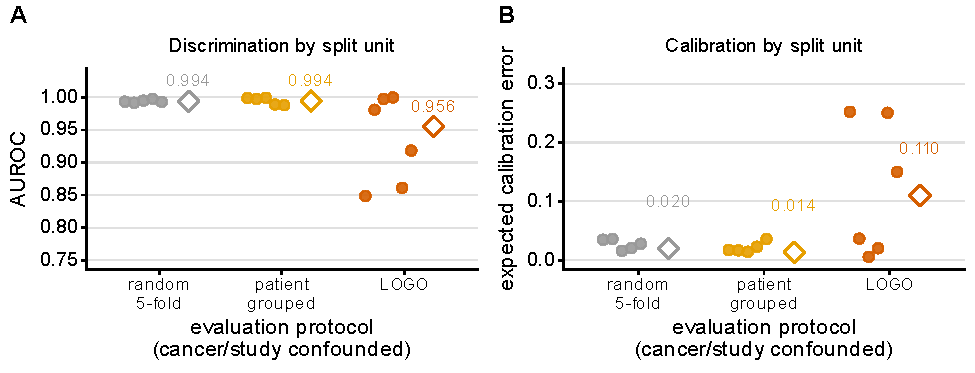
\includegraphics[width=0.92\linewidth]{figures/b28_F5_protocol.pdf}
\caption{Performance depends on the held-out unit. Filled points show
five sample-CV folds, five true-patient folds or six LOGO cohorts;
open diamonds show separately computed pooled metrics. (A) AUROC.
(B) Ten-bin ECE. The pooled values are not averages of the individual
fold values. Fold scatter is descriptive, not a confidence interval;
training sets overlap. Cancer type and study are confounded.}
\label{fig:protocol}
\end{figure}

\subsection{Small pooled sensitivity differences can hide cohort changes}

Full-dataset-median XGBoost has macro/pooled LOGO AUROC 0.9326/0.9543,
compared with 0.9343/0.9555 for training-fold medians. Its pooled ECE
is 0.1144, versus 0.1100. The pooled AUROC change of $-0.00125$ is
small, but CCRCC changes by $+0.00249$ and UCEC by $-0.00693$.
This diagnostic does not justify leaking held-out feature values or
claim that imputation is immaterial in other datasets.

Training-fold-imputed and standardized L2 logistic regression has
macro/pooled AUROC 0.9341/0.9556 and pooled ECE 0.0797. Its pooled
AUROC is only 0.00010 higher than XGBoost, yet CCRCC improves by
0.05520 and PDAC declines by 0.10434 (Figure~\ref{fig:sensitivity}).
Pooled agreement therefore does not imply model-family invariance.
These are matched-cohort sensitivity comparisons, without a claim of
statistical significance for any single cohort's change. SI Tables~S4--S6
retain the cohort-resolved mapping, L2 and deliberately leaky-median
outcomes under the definitions in SI Section S4. All six L2 LOGO fits
converged in 12--44 iterations under the executed 500-iteration limit
(SI Table~S8 and Section S6); convergence does not establish predictive
superiority.

\begin{figure}[tbp]
\centering
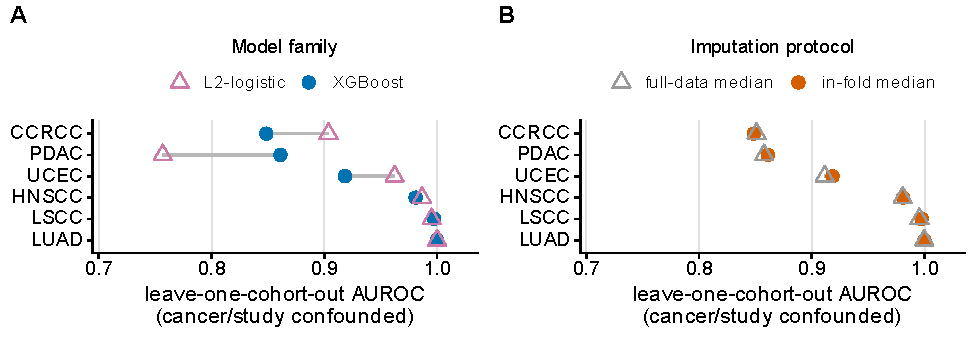
\includegraphics[width=0.92\linewidth]{figures/b28_F6_sensitivity.pdf}
\caption{Cohort-resolved model and imputation sensitivities. (A) XGBoost
versus L2 logistic regression, with training-fold imputation in both and
training-fold standardization for L2. CCRCC AUROC changes from 0.8485
to 0.9037 and PDAC from 0.8610 to 0.7567. (B) Training-fold versus
deliberately full-dataset medians for XGBoost, using identical outer
folds. The same AUROC scale is used in both panels. No interval or
significance claim is assigned to these single-fold comparisons.
Cancer type and study are confounded.}
\label{fig:sensitivity}
\end{figure}

\begin{figure}[tbp]
\centering
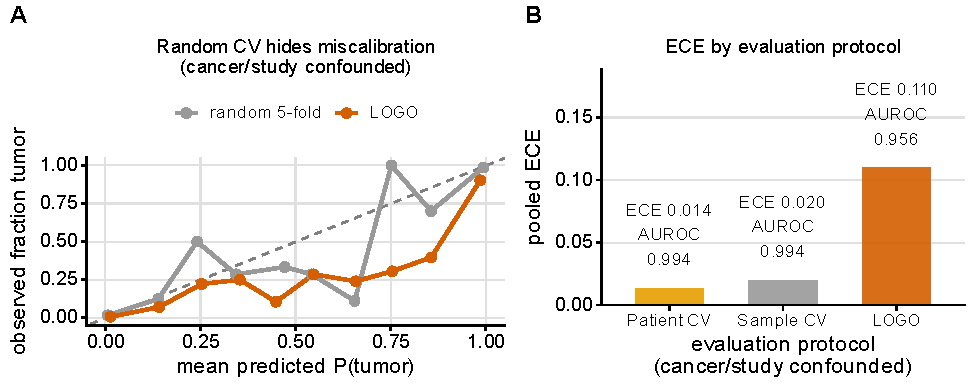
\includegraphics[width=\linewidth]{figures/b28_F3_calibration.pdf}
\caption{Cohort transfer has greater calibration error than cohort-mixing
CV. (A) Mean probability versus observed tumor fraction in ten equal-width
bins; the dashed line denotes perfect calibration. (B) Pooled ECE for
sample CV (0.0199), patient CV (0.0135) and LOGO (0.1100), with pooled
AUROC also shown. ECE uses each bin's sample mass, not equal bin weights.
This is a protocol contrast among confounded cancer/study cohorts.}
\label{fig:calibration}
\end{figure}

\subsection{Confidence-ranked abstention changes cohort composition}

Ranking pooled LOGO predictions by confidence raises retained accuracy
from 0.8497 at full coverage to 119/119 at 10\% requested coverage
(Figure~\ref{fig:abstention}). The top-confidence set contains 52 LUAD,
55 LSCC, six CCRCC, four HNSCC, two PDAC and no UCEC samples.
LUAD and LSCC together comprise 107/119 retained cases. The gain is
therefore accompanied by strong selection of easier cohorts, but the
composition alone does not identify how much improvement comes from
between-cohort selection versus within-cohort case ranking. In particular,
PDAC is not entirely absent from the retained set, contrary to the
historical result. The complete composition is given in
Table~\ref{tab:cohortcomp}.

Selective classification \citep{GeifmanSelective} and calibration answer
different questions. This retrospective curve does not repair
probability calibration, validate a deployment threshold, or ensure
reliability on a new PDAC- or UCEC-like population. Neither 119/119
correct retained predictions nor their pooled composition supplies a
clinical performance guarantee.

\begin{table}[tbp]
\centering
\caption{Cohort fractions in the confidence-ranked retained set.
Rows use the same stored LOGO predictions as the accuracy curve.
Requested coverage is rounded down to an integer retained count.}
\label{tab:cohortcomp}
\small
\begin{tabular}{lrrrrrrr}
\hline
Coverage & $n$ & CCRCC & LUAD & UCEC & HNSCC & LSCC & PDAC \\
\hline
\tableinput{tables/coverage_rows.tex}
\hline
\end{tabular}
\end{table}

\begin{figure}[tbp]
\centering
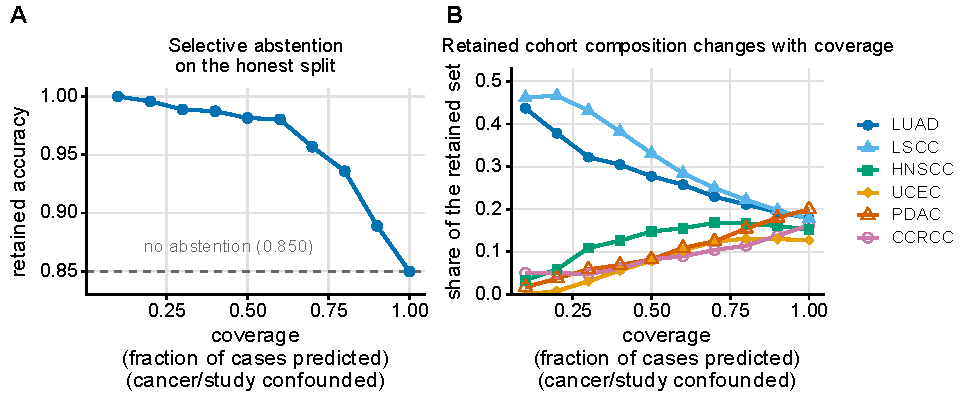
\includegraphics[width=\linewidth]{figures/b28_F4_riskcoverage.pdf}
\caption{Retained accuracy and retained populations change together.
(A) Accuracy among the highest-confidence LOGO predictions; the dashed
line is full-coverage accuracy 0.8497. (B) Cohort fractions in the same
sets. At 10\% coverage, LUAD and LSCC account for 52/119 and 55/119
samples; PDAC contributes 2/119 and UCEC contributes none. The curves
do not isolate within-cohort triage effects or validate an operational
abstention rule. Cancer type and study are confounded.}
\label{fig:abstention}
\end{figure}

\subsection{A specific recalibration procedure has cohort-dependent effects}

On the corrected outer LOGO predictions, split-half temperature scaling
reduces pooled ECE from 0.1100 to 0.0845 and Platt scaling to 0.0388.
Corresponding pooled Brier scores are 0.1135 before calibration, 0.0998
after temperature scaling and 0.0839 after Platt scaling. The cohort
breakdown in Table~\ref{tab:recal} shows uneven effects: for example,
Platt ECE falls from 0.2522 to 0.1303 on CCRCC but rises from 0.0203
to 0.0272 on LUAD.

The fitted temperatures range from 1.5506 to 2.0296 and all soften
the probabilities (Figure~\ref{fig:temperature}). This describes these
six fitted maps, not an intrinsic restriction of temperature scaling,
which can also sharpen probabilities when $T<1$. The calibration fit
uses inner two-/three-cohort predictors rather than the outer
five-cohort training regime. Consequently, heterogeneous benefit is a
result for this procedure, not proof that a single recalibration method
must fail under every transfer design. No held-out label was used to
fit the maps. The inner split construction and bounded temperature/Platt
fits are specified in SI Section S6, so this is a defined recalibration
procedure rather than an unspecified post-hoc correction.

\begin{figure}[tbp]
\centering
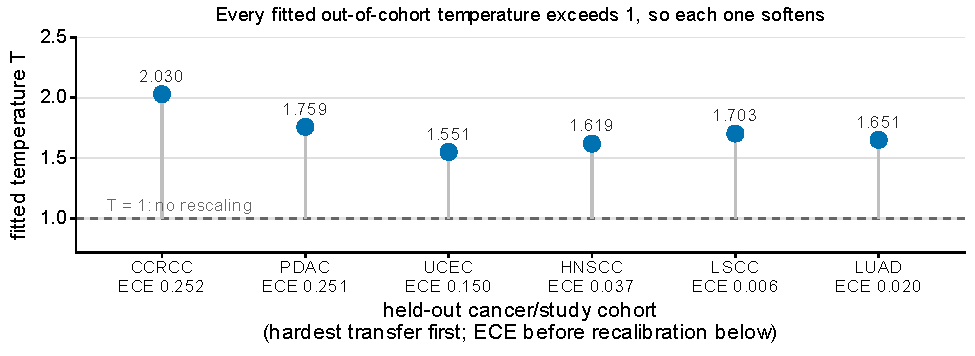
\includegraphics[width=\linewidth]{figures/b28_F7_temperature.pdf}
\caption{Temperatures fitted without outer held-out labels. All six
estimated temperatures exceed one in this analysis; the dashed line
denotes no rescaling. The printed ECE values are before recalibration.
The calibration predictors trained on two or three cohorts, while the
outer predictor trained on five. These maps therefore evaluate one
specified inner/outer procedure. Per-cohort outcomes and the Platt
alternative are in Table~\ref{tab:recal}. Cancer type and study are
confounded.}
\label{fig:temperature}
\end{figure}

\begin{table}[tbp]
\centering
\caption{Ten-bin ECE for the same outer LOGO predictions before and after
the specified split-half recalibration procedure. Each cohort has its
own map fitted using other cohorts only; pooled ECE is recomputed after
concatenation, not averaged over these rows.}
\label{tab:recal}
\begin{tabular}{lrrr}
\hline
Cohort & Before & Temperature & Platt \\
\hline
\tableinput{tables/recalibration_rows.tex}
\hline
\end{tabular}
\end{table}

\subsection{What the protocol contrast does not identify}

The study does not identify a biological or technical fraction of the
observed transfer performance. Each primary group corresponds to a
distinct cancer/study cohort; the source metadata do not establish that
each is a single acquisition batch. An observed sample/patient-versus-cohort
contrast can motivate choosing a relevant evaluation unit without
identifying why an individual cohort is hard.

The separately recorded OV side-study is retained as historical context:
its archived summary reports pooled plex-LOGO abundance AUROC 0.985, close to random five-fold
AUROC 0.987, with plex-LOGO ECE 0.046 and global-summary AUROC 0.951.
It has only 103 samples, including 19 normals distributed as one to
three per plex. It is one cancer type, a different feature table and a
different holdout unit. The reported near-zero protocol contrast is not a
prediction-replayed counterexample or a deconfounding test of the six-cohort result.
The current fixed six-cohort comparison does not establish a universal gap;
that restriction does not depend on treating the OV summary as verified new evidence.
These are retained historical summary values with checked source
provenance, not newly replayed OV predictions.

Numerical claims from historical six-cohort identification diagnostics,
synthetic shifts, representation transforms and the separate dual-platform
mapping are not used to strengthen the corrected primary conclusion.
Their assumptions and current evidence status are itemized in SI Section
S7, with the reproducibility boundary in Section S8. In particular, a
label-dependent residual
construction would not be a deployment evaluation, and a two-way
variance calculation on a confounded design would not by itself
identify biological and acquisition contributions. No pathway-enrichment
analysis was performed.
